\kommentar{Induktion} %Thema
  
\begin{karte}{Wie lautet das einfache Induktionsgesetz?}
	\begin{center}
		\huge
		$u_{i}(t)=-\dfrac{d \Phi}{d t}(t)$
	\end{center}
\end{karte}

\begin{karte}{Was sind die Primär- und die Sekundäreffekte der Induktion?}
	\flushleft
	\textbf{Primäreffekt:} Phänomen, dass ein elektrisches \\Feld($\rightarrow$ Spannung) entsteht, wenn sich das Magnetfeld ändert.\\
	\textbf{Sekundäreffekt:} Phänomen, welches eintrifft wenn durch die induzierte Spannung ein Strom fliessen kann. Dieser Strom verursacht ein Gegenfeld nach Lenz.\\[10pt]
	Der Primäreffekt tritt immer auf. Der Sekundäreffekt kann nur auftreten wenn ein Strom fliessen kann.
\end{karte}

\begin{karte}{Was ist elektromagnetische Induktion?}
	Eine induzierte Spannung durch ein zeitlich Änderung des Magnetfelds.\\
	\begin{equation*}
		u_{i}(t)=-\dfrac{d \Phi}{d t}(t)
	\end{equation*}
	\\[10pt]
	Ein Sekundäreffekt tritt dann ein wenn der Stromkreis geschlossen wird. Der fliessende Strom verursacht dann ein Gegenfeld. 
\end{karte}

\begin{karte}{Was ist Ruheinduktion?}
	Die zeitliche Änderung des Magnetfelds kommt von aussen. Die Geometrie in welcher eine Spannung induziert wird ruht.
\end{karte}

\begin{karte}{Wie wird im oder vom Magnetfeld Arbeit verrichtet?}
	Grundsätzlich wird eine Arbeit verrichtet, wenn etwas gegen eine Kraft bewegt wird.
	\begin{enumerate}
		\item Magnetische Flussänderung bewirken Wirbel im elektrischen Feld.
		\item Der Wirbel im elektrischen feld kann einen Strom verursachen. Dieser wiederum verursacht Wirbel im Magnetfeld.
		\item Die Magnetfelder überlagern sich, wirken einander entgegen.4
	\end{enumerate}
\end{karte}

\begin{karte}{Was ist totale Induktion?}
	Die totale Induktion oder Totalinduktion kann sowohl durch eine Bewegung innerhalb eines Magnetfelds, als auch durch zeitlich veränderliche Magnetfelder entstehen – je nach Sichtweise sind die Effekte schlicht ein und dieselben.\\
	Grundsätzlich kann somit gesagt werden, das die Totalinduktion durch die \textbf{Bewegungsinduktion} und die \textbf{Ruheinduktion} zusammengesetzt werden kann.
\end{karte}

\begin{karte}{Was bedeutet Selbstinduktion und Gegeninduktion?}
	Unter Selbstinduktion versteht man die Induktionswirkung eines Stromes auf seinen eigene Geometrie. Im Gegensatz dazu steht die Gegeninduktivität. Sie wird verursacht durch eine Stromänderung einer anderen Spule.
\end{karte}

\begin{karte}{Wie lautet das Ohmsche Gesetz von Induktivitäten?}	
	Der zeitlich veränderliche Strom $i_{L}$ verursacht ein Magnetfeld und damit einen sich ebenfalls zeitlich ändernden magnetischen Fluss $\Phi(t)$. An den Anschlussklemmen entsteht somit die Spannung $u_{L}(t)=\frac{d \Phi}{d t}(t)$.
	Daraus folgt dann das Ohmsche Gesetz von Induktivitäten:
	\begin{center}
		\huge
		$\dfrac{d i_{L}}{d t}(t)=\dfrac{u_{L}(t)}{L}$
	\end{center}
\end{karte}

\begin{karte}{Wie lautet der vollständige Durchflutungssatz?}
	\begin{center}
		$\displaystyle \oint_{C=\partial A} \vec{H} \cdot d \vec{l}=\int_{A}\left(\vec{J}_{\mathrm{frei}}+\frac{d \vec{D}}{d t}\right) \cdot d \vec{s} \quad \stackrel{\circ}{V}_{m}(t)=\Theta(t)+\frac{d \Psi}{d t}(t)$
	\end{center}
	Beispiel: Berechnung der Induktivität einer Ringkernspule\\[10pt]
	\begin{minipage}{0.4\textwidth}
		%Autor: Simon Walker
%Version: 1.0
%Datum: 10.11.2019

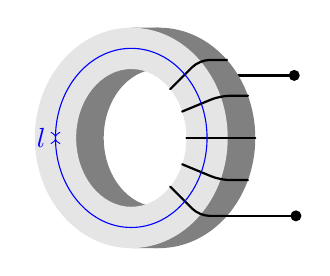
\begin{tikzpicture}[xscale=0.7, yscale=0.7, line cap=round, line join=round]
%\draw[help lines] (-2,-2) grid (3,2);
\draw [thick] (-45:1.75 and 2) -- ++(1.75,0) coordinate (a);
\draw [thick] (45:1 and 1.25)++(0,0.25) -- ++(2.25,0) coordinate (b);
\fill (a) circle [radius=.1] (b) circle [radius=.1];

\fill [gray, even odd rule] (0.5,0) 
  ellipse [x radius=1.75, y radius=2] ellipse [x radius=1, y radius=1.25];
\fill [gray] (0,2) rectangle ++(0.5, -0.25) (0,-2) rectangle ++(0.5, 0.25);
\fill [gray!20, even odd rule] 
  ellipse [x radius=1.75, y radius=2] ellipse [x radius=1, y radius=1.25];
\foreach \i in {-45,-22.5,...,45}
  \draw [thick, rounded corners=0.125cm] 
    (\i:1 and 1.25) -- (\i:1.75 and 2) -- +(0.5,0);
 
\draw [blue] ellipse [x radius=1.375, y radius=1.625];
\draw [blue, >-<] (-1.375, -0.11) -- (-1.375, 0.11);
\node [blue, left] at (-1.375, 0) {$l$};
 
\end{tikzpicture}

	\end{minipage}
	\begin{minipage}{0.6\textwidth}
			$L = N \cdot \frac{\Phi}{I}$\\
			\noindent\hspace*{3mm}
			$\Phi = B \cdot A$\\
			\noindent\hspace*{6mm} 
			$B = \mu \cdot H$\\
			\noindent\hspace*{9mm} 
			$H \cdot l = N \cdot I \rightarrow H = \frac{N \cdot I}{l}$\\
			\noindent\hspace*{6mm} 
			$B = \mu \cdot H = \frac{\mu \cdot N \cdot I}{l}$\\
			\noindent\hspace*{3mm}
			$\Phi = B \cdot A = \frac{A\mu \cdot N \cdot I}{l}$\\
			$L = N \cdot \frac{\Phi}{I} = \frac{A\mu \cdot N^2}{l}$
	\end{minipage}
	
\end{karte}

\begin{karte}{Wie wird die Induktivität einer Zylinderspule berechnet?}
	\flushleft
	Das Feld innerhalb einer Zylinderspule kann als Homogen betrachtet werden.\\[5pt]
	\begin{minipage}{0.37\textwidth}
		%Autor: Simon Walker
%Version: 1.0
%Datum: 10.11.2019

\begin{tikzpicture}[
  x=8mm,
  y=cos(30)*8mm,
  z={(0, -sin(30)*8mm)},
]
	\def\cylrad{1}% Zylinder Radius
	\def\cylht{5.5} %Zylinder Höhe
	\def\anzWind{10} %Anzahl Windungen (min 3)
	
	
	
	\draw[ultra thick] %Windungen Hinten
	\foreach \y in {\cylht/(2*\anzWind), 3*\cylht/(2*\anzWind),..., (((2*\anzWind-3)*\cylht)/(2*\anzWind))+0.1} 
	{
	 	plot[smooth, samples=25, variable=\t, domain=0:180]
	 	({-cos(\t)*\cylrad*1.1},
	 	{\y*0.8 + \cylht*0.1 + \t*(\cylht*0.8)/(360*\anzWind)},
	 	{-sin(\t)*\cylrad})
	}

	% Letzte Windung anders
	plot[smooth, samples=12, variable=\t, domain=0:90]
	(({-cos(\t)*\cylrad*1.1},
	{((2*\anzWind-1)*\cylht/(2*\anzWind))*0.8 + \cylht*0.1 + \t*(\cylht*0.8)/(360*\anzWind)},
	{-sin(\t)*\cylrad})
	-- ++(\cylrad*2, 0) coordinate(b);
	
	
	
	%%%%%%%%%%%%%%%%%%%%%%%%%%%%
	%Zylinder Farbig hinterlegen
	%%%%%%%%%%%%%%%%%%%%%%%%%%%%
	\filldraw [gray!25] (-\cylrad, \cylht) -- (-\cylrad, 0) -- (\cylrad, 0) -- (\cylrad, \cylht) -- (-\cylrad, \cylht);
  	%Boden
	\filldraw [gray!25] (0,0) ellipse [x radius=\cylrad, y radius=0.5\cylrad];
	%Deckel
	\filldraw [gray!10] (0,\cylht) ellipse [x radius=\cylrad, y radius=0.5\cylrad];
  
	\draw %Rand Zeichnern
	(-\cylrad, \cylht) -- (-\cylrad, 0) --
    plot[smooth, samples=25, variable=\t, domain=180:360]
      ({cos(\t)*\cylrad}, 0, {-sin(\t)*\cylrad}) --
    (\cylrad, \cylht)
    plot[smooth cycle, samples=51, variable=\t, domain=0:360]
      ({cos(\t)*\cylrad}, \cylht, {-sin(\t)*\cylrad});
	\draw[densely dashed] % Boden Hinten
	plot[smooth, samples=9, variable=\t, domain=0:180]
      ({cos(\t)*\cylrad}, 0, {-sin(\t)*\cylrad});
      
    %%%%%%%%%%%%%%%%%%%%%%
    %Windungen vorne  
    %%%%%%%%%%%%%%%%%%%%%%
	\draw[ultra thick] 
	%Erste Windung anders
	plot[smooth, samples=25, variable=\t, domain=360:270]
	({-cos(\t)*\cylrad*1.1},
	{\cylht*0.1 + (\t-180)*(\cylht*0.8)/(360*\anzWind)},
	{-sin(\t)*\cylrad}) -- ++(\cylrad*2, 0) coordinate(a);
	%Restliche Windungen
	\draw [ultra thick]
    \foreach \y in {\cylht/\anzWind, 2*\cylht/\anzWind,..., (\anzWind-1)*\cylht/\anzWind+0.1} {
      plot[smooth, samples=25, variable=\t, domain=180:360]
        ({-cos(\t)*\cylrad*1.1},
        {\y*0.8 + \cylht*0.1 + (\t-180)*(\cylht*0.8)/(360*\anzWind)},
        {-sin(\t)*\cylrad})
    };
	
	\fill (a) circle [radius=.1] (b) circle [radius=.1];
	
	\draw [thick, blue, <->] (-\cylrad*1.5, 0) -- (-\cylrad*1.5, \cylht);
	\node [blue, left] at (-\cylrad*1.5, \cylht/2) {\large $l$};
	
	\draw [thick, blue, ->] (0, \cylht, 0) -- (\cylrad/1.415, \cylht, -\cylrad/1.415);
	\node [blue, above] at (0, \cylht, 0) {\large $r$};
	
   
\end{tikzpicture}

	\end{minipage}
	\begin{minipage}{0.6\textwidth}
		$L = N \cdot \frac{\Phi}{I}$\\
		\noindent\hspace*{3mm}
		$\Phi = B \cdot A \quad \rightarrow \quad A = r^2\cdot\pi$ \\
		\noindent\hspace*{6mm} 
		$B = \mu \cdot H$\\
		\noindent\hspace*{9mm} 
		$H \cdot l = N \cdot I \rightarrow H = \frac{N \cdot I}{l}$\\
		\noindent\hspace*{6mm} 
		$B = \mu \cdot H = \frac{\mu \cdot N \cdot I}{l}$\\
		\noindent\hspace*{3mm}
		$\Phi = B \cdot A = \frac{A\mu \cdot N \cdot I}{l}$\\[5pt]
		$\boxed{L = \dfrac{A \cdot \mu \cdot N^2}{l}}$
	\end{minipage}
\end{karte}

\begin{karte}{Wie moddeliert man einen idealen Übertrager (Transformator)?}
	\flushleft
	\begin{minipage}{0.45\textwidth}
		%Autor: Simon Walker
%Version: 1.0
%Datum: 10.11.2019

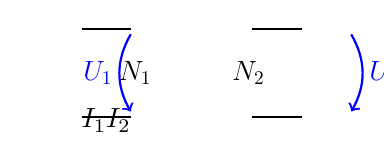
\begin{tikzpicture}[thick,scale=0.7, every node/.style={scale=0.7}]
	%\draw[help lines] (0,0) grid (4, 2);
	
	\tzTransformator{2}{1}{}
	\draw (0, 1-0.8) -- (2-1.1, 1-0.8);
	\draw (0, 1+0.8) -- (2-1.1, 1+0.8);
	\draw (4, 1-0.8) -- (2+1.1, 1-0.8);
	\draw (4, 1+0.8) -- (2+1.1, 1+0.8);
	
	\node[left] at (2-0.6, 1) {\Large $N_1$};
	\node[right] at (2+0.6, 1) {\Large $N_2$};
	
	\tzCurrent{0.5}{1+0.8}{$I_1$}{r}{a}
	\tzCurrent{4-0.5}{1+0.8}{$I_2$}{l}{a}
	
	\draw [->,thick ,blue] (4, 1+0.8-0.1) to [out=-60, in=60] (4, 1-0.8+0.1); 
	\node [blue, left] at (-0.2, 1) {\Large $U_1$};
	
	\draw [->,thick ,blue] (0, 1+0.8-0.1) to [out=-120, in=120] (0, 1-0.8+0.1); 
	\node [blue, right] at (4.2, 1) {\Large $U_2$};
	
\end{tikzpicture}

	\end{minipage}
	\begin{minipage}{0.52\textwidth}
	Ein Idealer Übertrager zeichnet sich dadurch aus, das insbesondere die Eingangsleistung gleich gross ist wie die Ausgangsleistung. $P_{in} = P_{out}$
	\end{minipage}\\[10pt]
	Zudem gelten Folgende Gleichungen:
	\begin{equation*}
		\begin{array}{lcl}
		{\color{red}{I_1}} = \dfrac{\color{red}{I_2}}{ü} & \hspace{15pt} &
		{\color{blue}{U_2}} = \dfrac{{\color{blue}{U_1}}}{ü}\\ \vspace{1pt}\\
		{\color{blue}{U_1}} = {\color{blue}{U_2}} \cdot ü & \hspace{15pt} & 
		\dfrac{{\color{blue}{U_1}}}{{\color{red}{I_1}}} = \dfrac{{\color{blue}{U_2}} \cdot ü}{\color{red}{I_2}}/ü = ü^2\cdot R_L\\
		\end{array}
	\end{equation*}
	
\end{karte}

\begin{karte}{Wie lauteten die Transformatoren Gleichungen?}
	\large
	\begin{equation*}
		\left[\begin{array}{c} U_1 \\ U_2 \end{array}\right] = 
		\dfrac{d}{dt}\left[ \begin{array}{cc} L_1 & M \\ M & L_2 \end{array} \right]
		\left[ \begin{array}{c} I_1 \\ I_2 \end{array} \right]
	\end{equation*}
	\begin{equation*}
	\left[\begin{array}{c} \underline{U}_1 \\ \underline{U}_2 \end{array}\right] = 
	j\omega \left[ \begin{array}{cc} L_1 & M \\ M & L_2 \end{array} \right]
	\left[ \begin{array}{c} \underline{I}_1 \\ \underline{I}_2 \end{array} \right]
	\end{equation*}
	\centering
	%Autor: Simon Walker
%Version: 1.1
%Datum: 06.01.2020

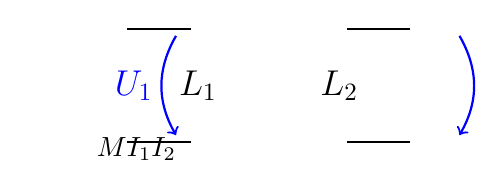
\begin{tikzpicture}[thick,scale=0.9, every node/.style={scale=0.9}]
	%\draw[help lines] (0,0) grid (4, 2);
	
	\tzTransformator{2}{1}{$M$}
	\draw (0, 1-0.8) -- (2-1.1, 1-0.8);
	\draw (0, 1+0.8) -- (2-1.1, 1+0.8);
	\draw (4, 1-0.8) -- (2+1.1, 1-0.8);
	\draw (4, 1+0.8) -- (2+1.1, 1+0.8);
	
	\node[left] at (2-0.6, 1) {\Large $L_1$};
	\node[right] at (2+0.6, 1) {\Large $L_2$};
	
	\tzCurrent{0.5}{1+0.8}{$I_1$}{r}{a}
	\tzCurrent{4-0.5}{1+0.8}{$I_2$}{l}{a}
	
	\draw [->,thick ,blue] (4, 1+0.8-0.1) to [out=-60, in=60] (4, 1-0.8+0.1); 
	\node [blue, left] at (-0.2, 1) {\Large $U_1$};
	
	\draw [->,thick ,blue] (0, 1+0.8-0.1) to [out=-120, in=120] (0, 1-0.8+0.1); 
	\node [blue, right] at (4.2, 1) {\Large $U_2$};
	
\end{tikzpicture}

\end{karte}

\begin{karte}{Was unterscheidet ideale und reale Kopplung?}
	\begin{itemize}
		\item Ideale Kopplung:\\
		$ M = \sqrt{L_1 \cdot L_2} $
		\item Reale Kopplung:\\
		$ M = k \cdot \sqrt{L_1 \cdot L_2} $
		\item Der Kopplungsfaktor $k$ kommt von dem Streufeld. Je mehr Streufeld desto kleiner ist $k$.
	\end{itemize}
\end{karte}

\begin{karte}{Welche Verluste können Transformatoren aufweisen?}
	\begin{itemize}
		\item Kupferverluste vor allem auf der Seite mit der höheren Anzahl an Windungen und kleineren Leiterquerschnitt.
		\item Magnetisierungsverluste. (Wegen der Hysterese) Es muss mehr Energie für das Aufbauen des Magnetfelds aufgewendet werden als beim Abbauen wider frei wird.
		\item Wirbelströme.
	\end{itemize}
\end{karte}

\begin{karte}{Was sind Hysterese Verluste und wie sind diese zu Erklären?}
	\begin{minipage}{0.49\textwidth}
		%Autor: Simon Walker
%Version: 1.0
%Datum: 14.11.2019
%Grundgrafik von OSjerick (tex.stackexchange.com) https://tex.stackexchange.com/questions/275192/hysteresis-loop

\begin{tikzpicture}%[thick,scale=0.7, every node/.style={scale=0.7}]
	\begin{axis}[very thick,
	             samples = 50,
	             xlabel = H,
	             ylabel = B,
	             xmin = -5,
	             xmax = 5,
	             ymin = -3,
	             ymax = 3,
	             axis x line = middle,
	             axis y line = middle,
	             ticks = none,
	             width=5cm,
	             height=5cm]
	    \addplot[dashed] plot (\x, 2);
	    \addplot[dashed] plot (\x,-2);
	    \addplot[red, name path=A] plot (\x, {4/(1 + exp(-1.7*\x+3))-2});
	    \addplot[red, name path=B] plot (\x, {4/(1 + exp(-1.7*\x-3))-2});
	    \addplot[red!20] fill between[of=A and B];
	\end{axis}
\end{tikzpicture}

	\end{minipage}
	\begin{minipage}{0.49\textwidth}
		\textbf{Formel Energiedichte:}\\[10pt]
		$
			w_m = \frac{1}{2} \cdot \vec{B} \cdot \vec{H}
		$
	\end{minipage}
	Beim aufbauen des Magnetfelds muss, dank der Hysterese, mehr Energie aufgewendet werden, als beim abbauen wider frei gesetzt wird. Dieser Verlust ist proportional zur Fläche, welche durch die Hysteresekurve eingeschlossen wird. Dieser Verlust lässt sich über die Energiedichte berechnen.
\end{karte}

\begin{karte}{Wie Verursachen Wirbelströme im Transformator Verluste und wie kann man diese minimieren?}
	%Autor: Simon Walker
%Version: 1.0
%Datum: 15.11.2019

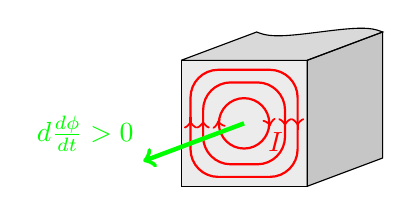
\begin{tikzpicture}[
x=8mm,
y=8mm,
z={(0.8*8mm, 0.3*8mm)},
]
	
	
	%%%%%%%%%%%%%%%%%%%%%%%%%%%%
	%Zylinder Farbig hinterlegen
	%%%%%%%%%%%%%%%%%%%%%%%%%%%%
	
	\filldraw [gray!15] (-1,-1,0) rectangle (1,1,0);
	\filldraw [gray!30] (-1,1,0) -- (1,1,0) -- (1,1,1.5) -- 
		plot[smooth, samples=25, variable=\t, domain=0:360]
		({1-(2*\t/360)},
		{1},
		{1.5+ 0.2*sin(\t)})
	-- (-1,1,1.5) -- (-1,1,0);
	\filldraw [gray!45] (1,-1,0) -- (1,1,0) -- (1,1,1.5) -- (1,-1,1.5) -- (1,-1,0);
	
	\draw (-1,-1,0) rectangle (1,1,0);
	\draw (-1,1,0) -- (1,1,0) -- (1,1,1.5) -- 
	plot[smooth, samples=50, variable=\t, domain=0:360]
	({1-(2*\t/360)},
	{1},
	{1.5+ 0.2*sin(\t)})
	-- (-1,1,1.5) -- (-1,1,0);
	\draw (1,-1,0) -- (1,1,0) -- (1,1,1.5) -- (1,-1,1.5) -- (1,-1,0);
	
	\draw [red, thick] (0, 0, 0) circle [radius=0.4];
	%\draw (x,y) arc (start:stop:radius);
	\draw[red, thick, -<] (170 : 0.4)  arc(170:190:0.4);
	\draw[red, thick, -<] (-10 : 0.4)  arc(-10:10:0.4);
	
	\draw [red, thick, rounded corners=10] (-0.65, -0.65, 0) rectangle (0.65, 0.65, 0);
	\draw [red, thick, -<] (-0.65, 0.1, 0) -- (-0.65, -0.08, 0);
	\draw [red, thick, -<] (0.65, -0.1, 0) -- (0.65, 0.08, 0);
	\draw [red, thick, rounded corners=10] (-0.85, -0.85, 0) rectangle (0.85, 0.85, 0);
	\draw [red, thick, -<] (-0.85, 0.1, 0) -- (-0.85, -0.08, 0);
	\draw [red, thick, -<] (0.85, -0.1, 0) -- (0.85, 0.08, 0);
	
	\node[red] at (0.5, -0.3, 0) {$I$};
	
	%\draw[red, thick, ->] (0,0 : 0.4)  arc[start angle=-10, end angle=0];
		
	\draw [green, ultra thick, ->] (0, 0, 0) -- (0, 0, -2);
	\node [above left, green] at (0, 0, -2) {$d\frac{d\phi}{dt}>0$};
      
      
%      %Hilfs Koordinaten System
%      \draw [->] (-3,0,0) -- (3,0,0);
%      \node [above] at (3,0,0) {x};
%      \draw [->] (0,-3,0) -- (0,3,0);
%      \node [above] at (0,3,0) {y};
%      \draw [->] (0,0,-3) -- (0,0,3);
%      \node [above] at (0,0,3) {z};
%   	
   
\end{tikzpicture}
\\[5pt]
	Ein sich änderndes Magnetfeld (in diesem Fall ist es zunehmend), Induziert ein Strom im Eisen. Dieser wiederum verursacht ein Magnetfeld welches der Änderung entgegenwirkt. (gemäss der Lenzschen Regel)\\[5pt]
	Deshalb wird in einem Transformator meistens ein geschichteter Eisenkern verwendet. Dieser lässt den Wirbelstrom nur in einer dünnen Scheibe fliessen. Dadurch ist der Wirbelstrom kleiner und kann somit weniger stark dem Feld entgegen wirken. 
\end{karte}

\begin{karte}{Wie können die Hystereseverluste im Leerlaufbetrieb gemessen werden?}
	%Autor: Simon Walker
%Version: 1.0
%Datum: 14.11.2019

\begin{tikzpicture}[thick,scale=0.7, every node/.style={scale=0.7}]
	%\draw[help lines] (0,0) grid (10, 5);
	
	
	\tzTransformator{5.5}{2.5}{$M$}
	\node[left] at (5.5-0.6, 2.5) {\Large $L_1$};
	\node[right] at (5.5+0.6, 2.5) {\Large $L_2$};
	
	\tzRV{3.5}{2.5}{}{} %RP
	\tzRH{2}{4}{}{} %RS1
	\tzRH{8}{4}{}{} %RS2
	
	
	\draw (5.5-1.1, 2.5+0.8) -- (5.5-1.1, 4) -- (2 + 0.7, 4); %Trafo RS1
	\draw (0, 4) -- (2-0.7, 4); %To RS1
	\draw (0, 1) -- (5.5-1.1, 1) -- (5.5-1.1, 2.5-0.8); %To Trafo
	\draw (5.5+1.1, 2.5+0.8) -- (5.5+1.1, 4) -- (8 - 0.7, 4); %Trafo RS2
	\draw (8+0.7 , 4) -- (9.5, 4); %to RS2
	\draw (9.5, 1) -- (5.5+1.1, 1) -- (5.5+1.1, 2.5-0.8); %To Trafo
	
	\draw (3.5, 4) -- (3.5, 2.5+0.7);
	\draw (3.5, 1) -- (3.5, 2.5-0.7);
	\tzKN{3.5}{4}
	\tzKN{3.5}{1}
	
	
	\tzCurrent{1}{4}{$i_1(t)$}{r}{a}
	
	\draw [->,thick ,blue] (9.5, 4-0.1) to [out=-60, in=60] (9.5, 1+0.1); 
	\node [blue, left] at (9.5, 2.5) {\Large $u_2(t)$};
	
\end{tikzpicture}
\\
	\begin{equation*}
		H(t) = \frac{N\cdot i_1(t)}{l}  
		\quad \& \quad 
		B(t) = \frac{\int u_2(t) dt}{A}
	\end{equation*}\\[2pt]
	$H(t)$ lässt sich durch den Durchflutungssatz berechnen.\\
	$B(t)$ lässt sich über die Induzierte Spannung berechnen.\\ 
\end{karte}

\begin{karte}{Wie äussert sich der Skin-Effekt und von Welchen Parameter hängt er ab?}
	\begin{minipage}{0.6\textwidth}
		\begin{itemize}
			\item Je höher die Frequenz, desto weniger Strom fliest der im Innern des Leiters. Und desto grösser wird dadurch der Widerstand, da die effektive Querschnittsfläche kleiner wird
			\item Die Eindringtiefe (Skin-Tiefe) ist wie folgt definiert:\\[5pt]
			\large
			$ \delta=\sqrt{\dfrac{2}{\omega \sigma \mu}} $
		\end{itemize}
	\end{minipage}
	\begin{minipage}{0.39\textwidth}
		%Grafik von Wikipedia (Public Domain) https://de.wikipedia.org/wiki/Skin-Effekt
		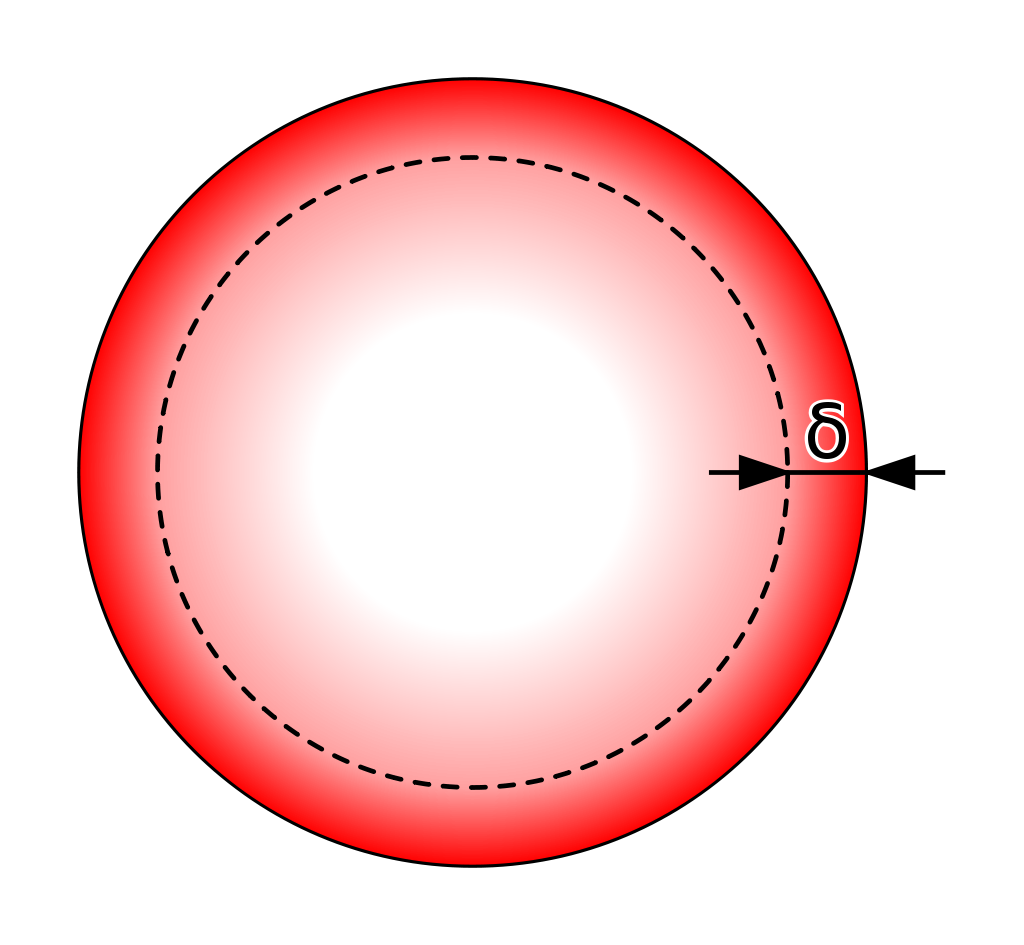
\includegraphics[width=\textwidth]{bilder/2_SkinEfekt.png}
	\end{minipage}
	
\end{karte}
